%%%%%% CMB-S4 Simulations and Data Analysis Chapter, Time-Ordered Data Procesing Section  %%%%%%%%%%%%%%%%
 
\section{Time-Ordered Data Processing}

\subsection{Overview}

The time-ordered data processing elements of the CMB simulation and analysis pipeline -- simulation, pre-processing and mission characterization, and map-making -- are grouped as a subset due to the unique computational challenges posed by the volume of data they must process.

\begin{figure}[htbp]
\centering
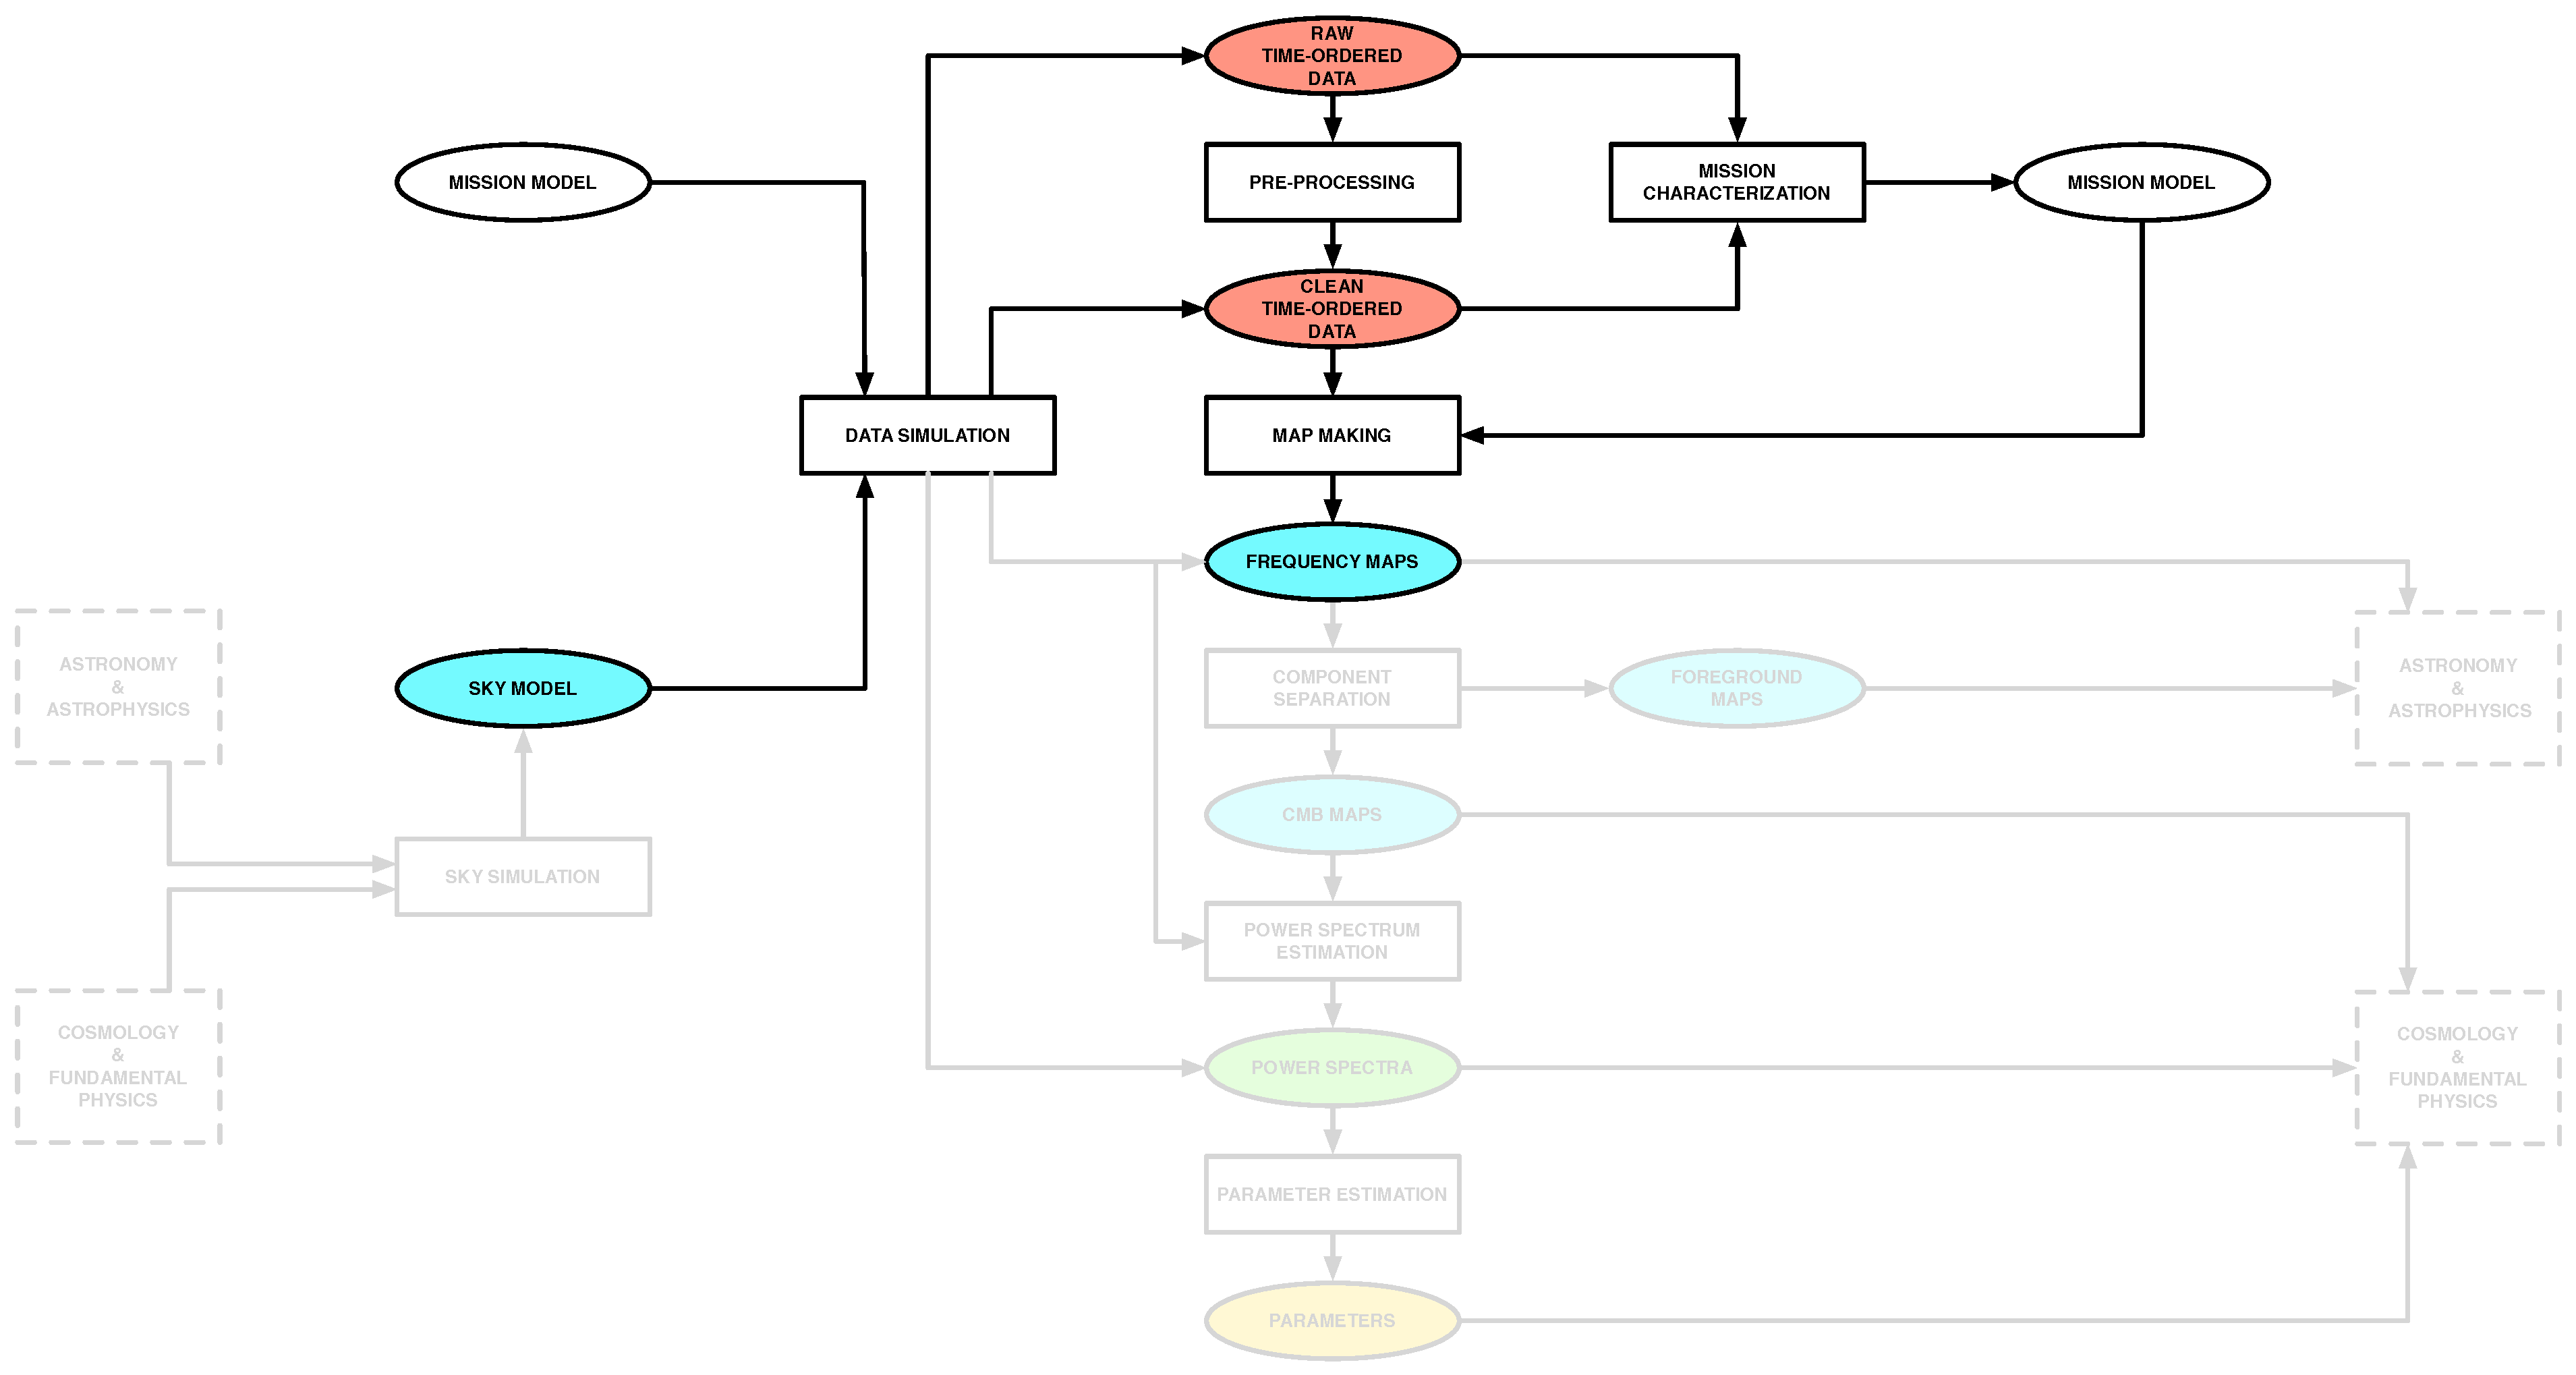
\includegraphics[width=1\textwidth]{Analysis/td}
\caption{The time-ordered data processing subset of the CMB simulation and data analysis pipeline}
\label{fig_td}
\end{figure}

\subsection{Simulation}

sky signal to readout

instrument - beam, bandpass, noise; calibration, electronics

observation -- pointing, polarization (hwp), flagging, atmosphere

V \& V for other TOD processing elements

\subsection{Pre-Processing and Mission Characterization}

systematics mitigation: filtering, template-subtraction, marginalization

mission model building: beam, noise, pointing

\subsection{Map-Making}

maximum likelihood

destriping

effective beam convolution

binning

\subsection{Computational Constraints}



The computational requirements here are for both capacity and capability. To support the iterative exploration of the time-ordered data required by the pre-processing and mission characterization steps we need many analysts to be able to process the full data simultaneously, with each seeing no worse than order 1-day turnaround time for their jobs to complete. Conversely, to support the massive Monte Carlo simulation and map-making required for percent level uncertainty quantification in the absence of a full data covariance matrix, we need to be able to perform occasional runs of up to $10^4$ realizations within the total cycles available to us.


As Figure \ref{fig_cmb_hpc_scaling} shows, the size of ground-based, balloon-borne and satellite CMB data sets exhibit exponential growth over a 40 year period. Moreover, for suborbital experiments the exponent exactly matches that of Moore's Law, where we us as a proxy the peak performance of the flagship high performance computing (HPC) system at the DOE's National Energy Research Scientific Computing (NERSC) Center at any epoch (this choice reflecting the widespread use of NERSC for CMB data analyses over the last 20 years). 



\begin{figure}[htbp]
\centering
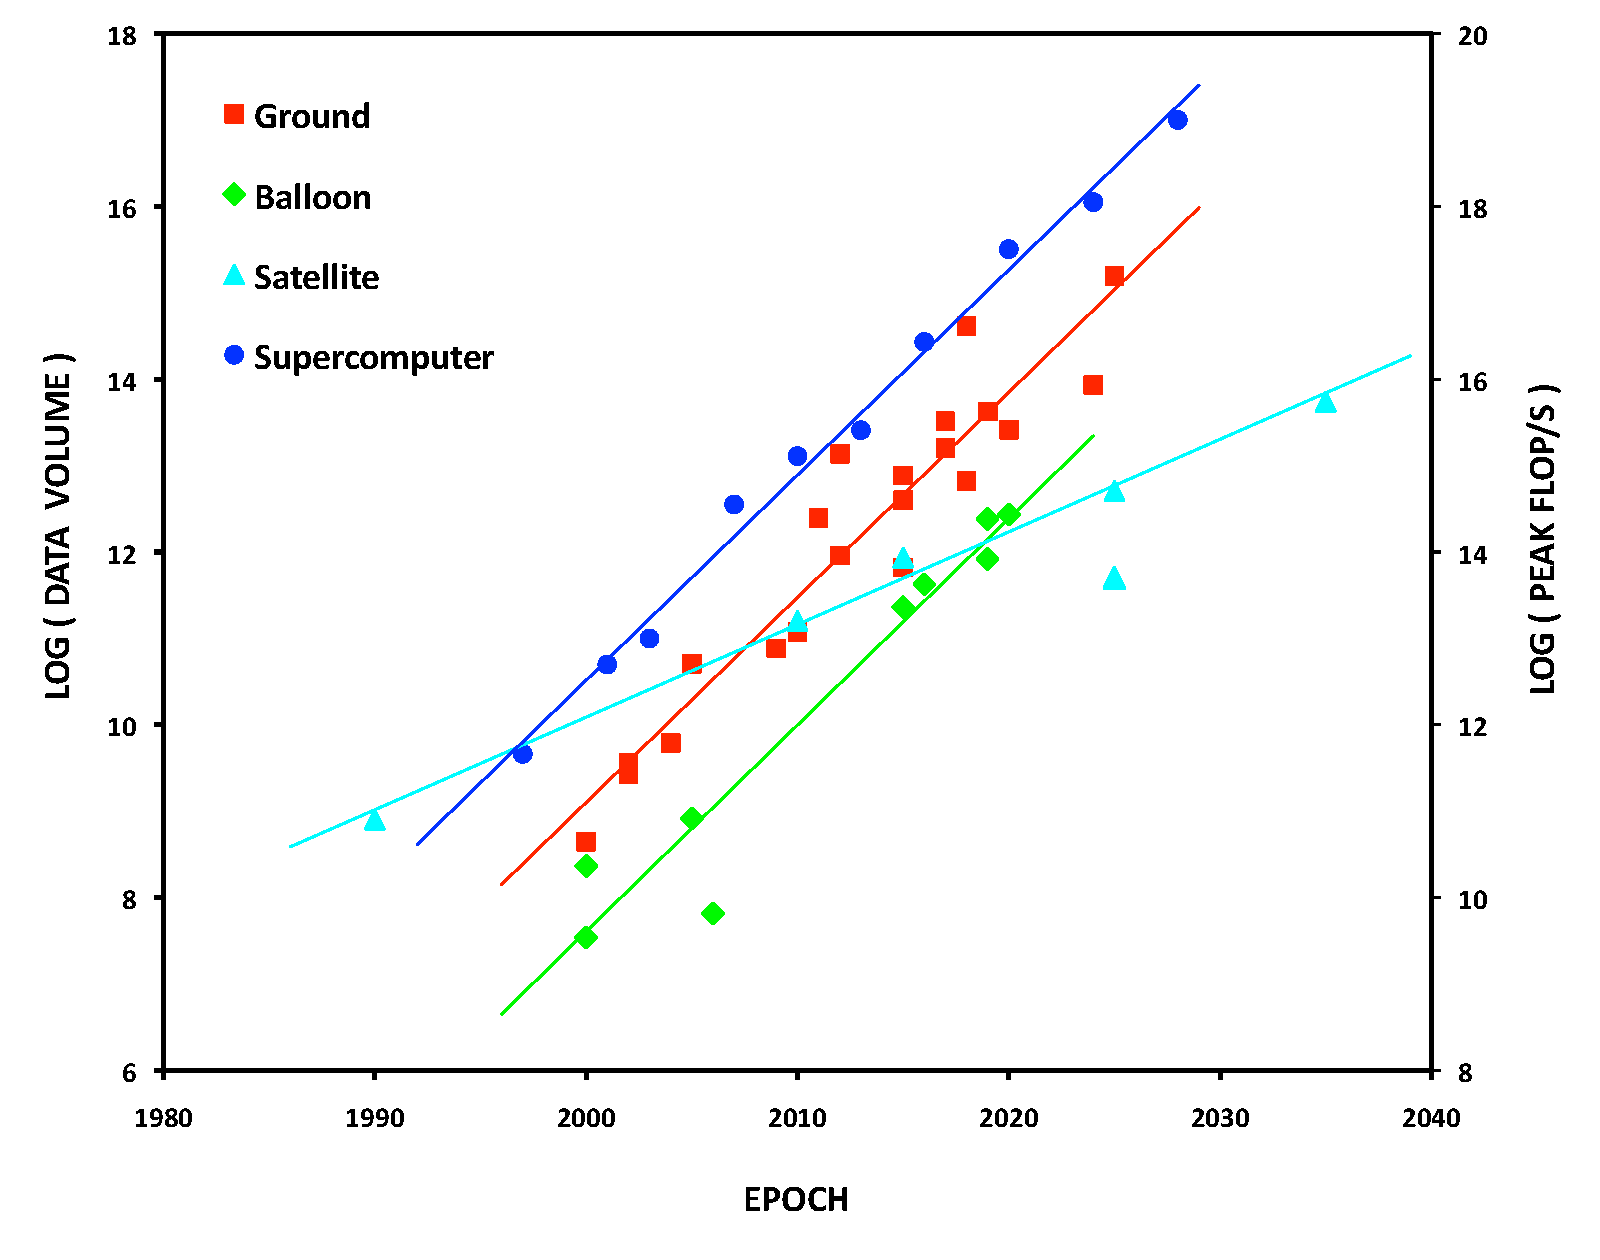
\includegraphics[width=0.5\textwidth]{Analysis/cmb_hpc_scaling}
\caption{Exponential growth of CMB time-ordered data volume and HPC capability: 1990 -- 2030.}
\label{fig_cmb_hpc_scaling}
\end{figure}


As noted above, the intractability of pixel-domain data covariance matrices pushes us to use Monte Carlo (MC) methods for uncertainty quantification and debiasing, and the computational cost of the data analysis is dominated by the generation and reduction of sufficient MC realizations of the data for the resulting statistical error to be subdominant (typically assumed to be $10^4$ realizations for percent level uncertainty). 


; specifically, all algorithmic and implementation choices we make must first and foremost be informed by their impact on computational tractability.


Key challenges:
\begin{itemize}
\item computational tractability due to data volume and complexity of next-generation supercomputers
\item mitigating raw data systematics and developing sufficient mission and data models
\end{itemize}


%\bibliography{cmbs4}

%%
%% Populate the .bib file with entries from SPIRES Bibtex (preferred)
%% or ADS Bibtex (if no SPIRES entry).
%%  SPIRES will also supply the CITATION line information; please include it.
%%


